\documentclass{beamer}
 
\usepackage[utf8]{inputenc}
\usepackage[english,russian]{babel}
\usepackage{graphicx}
\graphicspath{ {./pictures/} }
\usepackage{color}


\mode<presentation> {\usetheme{default}}
\setbeamertemplate{itemize items}[triangle]
 
\title[Distributed map-reduce]{Курсовой проект \\ \it{Фреймворк и файловая система для распределённой обработки больших данных в рамках концепции map-reduce}}

\author{Выборнов А.И,} % Your name
\institute[МГТУ ИУ-9] {
    МГТУ~им.~Н.~Э.~Баумана \\
    \medskip
    \text{art-vybor@ya.com}
}
\date{\today}

\begin{document}
%----------------------------------------------------------------------------------------
%    Title
%----------------------------------------------------------------------------------------
\begin{frame}
    \titlepage
\end{frame}

%----------------------------------------------------------------------------------------
%   Revierw
%----------------------------------------------------------------------------------------

\begin{frame}
\frametitle{Обзор} 
\tableofcontents 
\end{frame}

%----------------------------------------------------------------------------------------
%   Presentation
%----------------------------------------------------------------------------------------

\section{Постановка задачи}
    \begin{frame}
    \frametitle{Постановка задачи}
        \begin{itemize}
            \item Анализ требований и проектирование архитектуры системы. Реализация нераспределённого map-reduce. Решение проблемы RPC.
            \item Реализация распределённой файловой системы. Реализация фреймворка. Тестирование на примерах.
            
        \end{itemize} 
    \end{frame}

\section{Концепция map-reduce}
    \begin{frame}
    \frametitle{Зачем нужен map-reduce?}
        \begin{itemize}
            \item Обработка больших данных (Big Data).
            \begin{itemize}
                \item Вычисления превосходят возможности одной машины.  
                \item Данные не помещаются в памяти, необходимо обращаться к диску.
                \item Можно хранить много данных, но задержки и пропускная способность оборудования растут пропорционально данным.
            \end{itemize}
            \item Удобная абстракция для построения алгоритмов обработки больших данных.
            \item Устойчивость к отказам.            
        \end{itemize} 
    \end{frame}

    \begin{frame}
    \frametitle{Что такое map-reduce?}
        \begin{itemize}
            \item Структура (key, value) - пара (ключ, значение).
            \item Программирование представляет собой определение двух функций:
            \begin{itemize}
                \item $map: (key, value)\rightarrow[(key, value)]$
                \item $reduce: (key, [value])\rightarrow[(key, value)]$
            \end{itemize}
            \item Между стадиями $map$ и $reduce$ происходит группировка и сортировка данных.
            
        \end{itemize} 
    \end{frame}

    \begin{frame}
    \frametitle{Что такое map-reduce?}
        \begin{figure}[h!]
            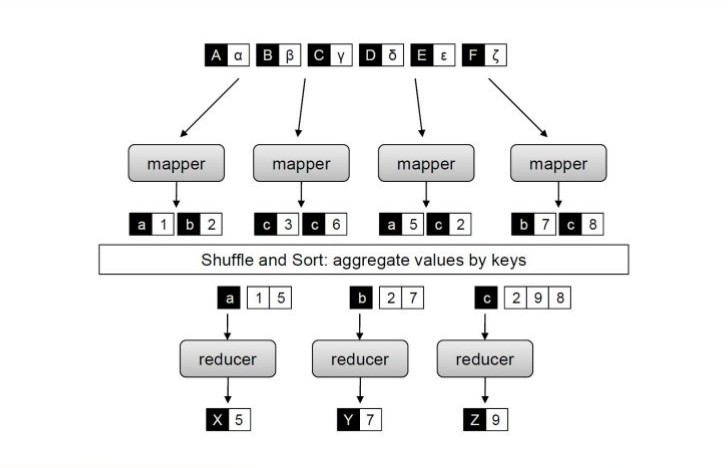
\includegraphics[scale=0.4]{mapreduce_lite.jpg}
        \end{figure}
    \end{frame}

    \begin{frame}
    \frametitle{А на самом деле}
        \begin{figure}[h!]
            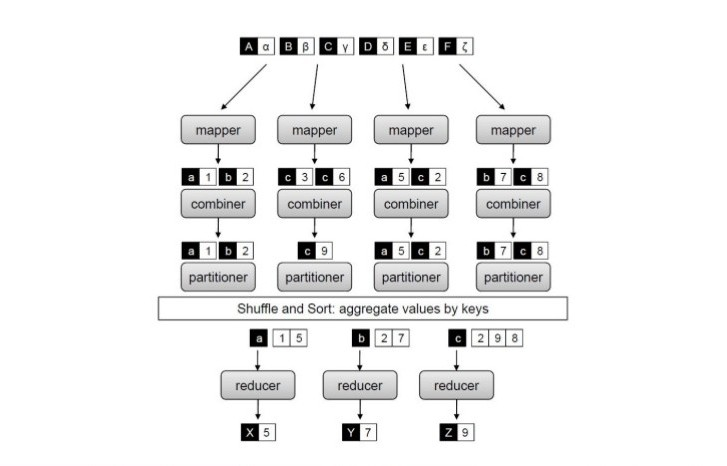
\includegraphics[scale=0.4]{mapreduce.jpg}
        \end{figure}
    \end{frame}
    

\section{Архитектура}
    \begin{frame}
    \frametitle{Архитектура распределённого map-reduce}
        \begin{figure}[h!]
            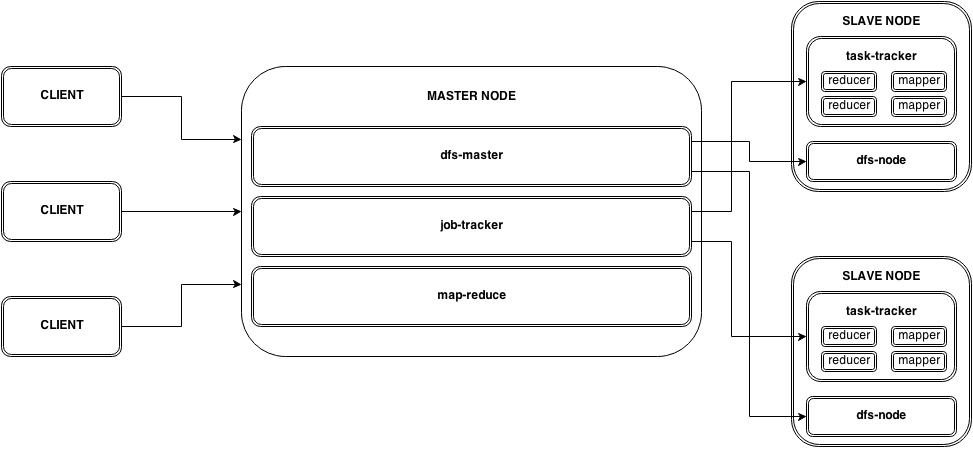
\includegraphics[scale=0.3]{map-reduce.png}
        \end{figure}
        
    \end{frame}

    \begin{frame}
    \frametitle{Архитектура распределённой файловой системы}
        \begin{figure}[h!]
            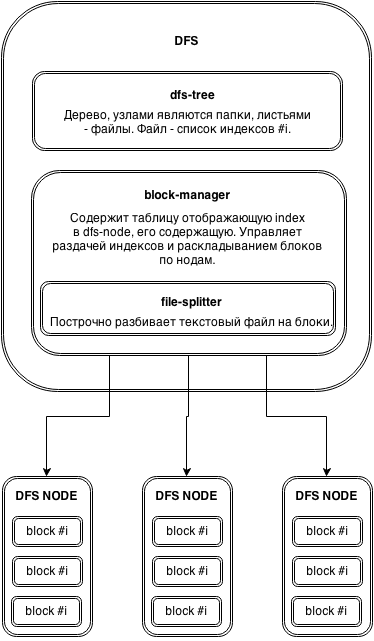
\includegraphics[scale=0.3]{dfs.png}
        \end{figure}
    \end{frame}

\section{Отчёт}
    \begin{frame}
    \frametitle{Что сделано}
        \begin{itemize}
            \item Разработаны архитектуры распределённых map-reduce и файловой системы.
            \item Реализован нераспределённый map-reduce, включающий в себя все этапы распределённого.
            \item Для реализации RPC была выбрана связка: ZeroMQ + Pickle.
            \item Реализована распределённая файловая система.
        \end{itemize} 
    \end{frame}

    \begin{frame}
    \frametitle{Что предстоит сделать}
        \begin{itemize}
            \item Развить существующую распределённую файловую систему.
            \item Реализовать распределённый map-reduce.
            \item Протестировать полученную систему на больших данных и проанализировать результаты.
        \end{itemize} 
    \end{frame}

\begin{frame}
    \titlepage
\end{frame}

\end{document}